\chapter{能量和动量}
\section{动能定理}

由Newton 第二定律可以推导出动能定理.对于任意的一个运动,我们可以使用微元法求出合外力对它做的总功.在每一个小部分,只要足够小,那这一小部分的运动就可以近似视为匀变速直线运动,而合力在运动方向的分力就是这一段``匀变速直线运动''的加速度来源.

\subsection{匀变速直线运动合外力做功}

由 Newton 第二定律 \eqref{eq:newton2}得

\begin{equation}
  F=ma
  \label{eq:newtonK}
\end{equation}

对上式左右同时乘以位移 $x$ ,再由匀变速直线运动位移与速度的关系 \eqref{eq:x-v} 得

\begin{gather}
  Fx=max \\
  Fx=\frac{1}{2}m\cdot 2ax\\
  Fx=\frac{1}{2}m(v^2-v_0^2)\\
  Fx=\frac{1}{2}mv^2-\frac{1}{2}mv_0^2\\
  W=\frac{1}{2}mv^2-\frac{1}{2}mv_0^2
\end{gather}

由上式定义动能$E_k=\frac{1}{2}mv^2$.

\subsection{任意情况下合外力做功}

\begin{figure}[H]
  \centering
  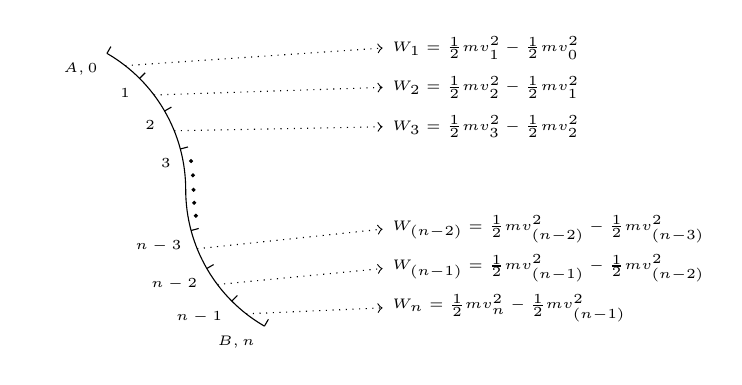
\begin{tikzpicture}
   \draw (0,0) arc (0:60:2); 
   \draw (0,0) arc (180:240:2);
   \draw (-2,0)+(60:2) node [anchor= north east]{\tiny $A,0$}--+(60:2.1);
   \draw (-2,0)+(45:2) node [anchor= north east]{\tiny $1$}--+(45:2.1);
   \draw (-2,0)+(30:2) node [anchor= north east]{\tiny $2$}--+(30:2.1);
   \draw (-2,0)+(15:2) node [anchor= north east]{\tiny $3$}--+(15:2.1);
   \draw[->,dotted] (-2,0)+(52:2)--+(4.5,1.8) node [anchor=west]{\tiny $W_1=\frac{1}{2}mv_1^2-\frac{1}{2}mv_0^2$};
   \draw[->,dotted] (-2,0)+(37:2)--+(4.5,1.3) node [anchor=west]{\tiny $W_2=\frac{1}{2}mv_2^2-\frac{1}{2}mv_1^2$};
   \draw[->,dotted] (-2,0)+(22:2)--+(4.5,0.8) node [anchor=west]{\tiny $W_3=\frac{1}{2}mv_3^2-\frac{1}{2}mv_2^2$};
   \filldraw (-2,0)+(10:2.1) circle [radius=0.5pt]; 
   \filldraw (-2,0)+(5:2.1) circle [radius=0.5pt]; 
   \filldraw (-2,0)+(0:2.1) circle [radius=0.5pt]; 
   \filldraw (2,0)+(185:1.9) circle [radius=0.5pt]; 
   \filldraw (2,0)+(190:1.9) circle [radius=0.5pt]; 
   \draw (2,0)+(195:2) node [anchor= north east]{\tiny $n-3$}--+(195:1.9);
   \draw (2,0)+(210:2) node [anchor= north east]{\tiny $n-2$}--+(210:1.9);
   \draw (2,0)+(225:2) node [anchor= north east]{\tiny $n-1$}--+(225:1.9);
   \draw (2,0)+(240:2) node [anchor= north east]{\tiny $B,n$}--+(240:1.9);
   \draw[->,dotted]  (2,0)+(202:2)--+(0.5,-0.5) node [anchor=west] {\tiny $W_{(n-2)}=\frac{1}{2}mv_{(n-2)}^2-\frac{1}{2}mv_{(n-3)}^2$};
   \draw[->,dotted]  (2,0)+(217:2)--+(0.5,-1) node [anchor=west]{\tiny $W_{(n-1)}=\frac{1}{2}mv_{(n-1)}^2-\frac{1}{2}mv_{(n-2)}^2$};
   \draw[->,dotted] (2,0)+(232:2)--+(0.5,-1.5) node [anchor=west]{\tiny $W_n=\frac{1}{2}mv_n^2-\frac{1}{2}mv_{(n-1)}^2$};
 \end{tikzpicture}
  \caption{动能定理}
  \label{fig:dongneng}
\end{figure}

在图 \ref{fig:dongneng} 中,质点从$A$ 点沿任意一条路线运动到 $B$ 点,为了求出这个过程中外力做的总功,我们将此路径划分为$n$ 份,则每一小段上可以视为匀变速直线运动.总功则是这 $n$ 段上的合外力的和.即

\begin{gather}
  W_1+W_2+\cdots +W_n =\frac{1}{2}mv_n^2-\frac{1}{2}mv_0^2
  \label{eq:dongneng1}
\end{gather}

当 $n\to \infty$ 时,则误差消失,将总功记为 $W$ , $v_n$ 记为 $v$ ,则动能定理表达为

\begin{equation}
  W=\frac{1}{2}mv^2-\frac{1}{2}mv_0^2
  \label{eq:dongneng2}
\end{equation}

经过上述论述,我们可以确定动能定理适用于一切情况,在推导过程中将每一小部分视为匀变速直线运动,然后再求和.但是,我们得出这个和为全过程中的总功,一般在使用时我们通常计算过程中每个力做的功然后再求和.即

\begin{equation}
  W=W_{f1}+W_{f2}+W_{f3}+\cdots 
  \label{eq:dongneng3}
\end{equation}

\section{功能原理}

在一个系统中,设除重力弹力之外的其它力做功为 $W_{\tiny\mbox{其}}$ 则,动能定理可以表达为

\begin{equation}
  W_{\tiny\mbox{其}}-\Delta E_p =\Delta E_k
  \label{eq:gnyl}
\end{equation}

将式 \eqref{eq:gnyl} 中的势能部分移项到等号右侧,同时考虑到机械能 $E=E_p+E_k$ 得功能原理为

\begin{equation}
  W_{\tiny\mbox{其}}=\Delta E
  \label{eq:gnyl1}
\end{equation}

式 \eqref{eq:gnyl1} 就是一般意义下的功能原理.它表明:一个系统中,除了重力弹力之外其它力做的功等于系统机械能的增加量.

\section{机械能守恒定律}

如果一个系统所受到的除重力弹力之外的力做功为零,则机械能守恒.也就是$W_{\tiny\mbox{其}}=0$ ,则式\eqref{eq:gnyl1} 为

\begin{gather}
  0=\Delta E \notag \\
  E_2=E_1
  \label{eq:jxnsh}
\end{gather}

式 \eqref{eq:jxnsh} 就是机械能守恒定律.一般而言在对一个系统列出动能定理时,要在表达式中列出具体的式子,如下

\begin{equation}
  mgh_1+\frac{1}{2}kx_1^2+\frac{1}{2}mv_1^2=mgh_2+\frac{1}{2}kx_2^2+\frac{1}{2}mv_2^2
  \label{eq:jxnshonly}
\end{equation}

如果一个系统有多个物体,则以具体数字表示各个物体,以``$^\prime$''号表示末态,不带撇号的量表示初态.则机械能守恒定律为

\begin{equation}
  E_1'+E_2'+\cdots +E_n'=E_1+E_2+\cdots +E_n
  \label{eq:jxnshmulti}
\end{equation}

\section{动量定理}

对于一个质点的做匀变速直线运动时我们可以由式 \eqref{eq:newton2}得到动量定理,重写 \eqref{eq:newton2}如下

\begin{gather}
  F=ma
  \label{eq:dongliang}
\end{gather}

将上式 \eqref{eq:dongliang} 左右同时乘以时间$t$ ,再代入匀变速直线运动速度与时间的关系 \eqref{eq:v-t} 计算如下

\begin{gather}
  Ft=m\cdot at \notag\\
  Ft=m(v-v_0) \notag \\
  Ft=mv-mv_0
  \label{eq:dldl}
\end{gather}

由式 \eqref{eq:dldl} 定义冲量为 

\begin{equation}
  I=Ft
  \label{eq:chongliang}
\end{equation}

注意:冲量是一个矢量,它的方向与所受力的方向相同,单位是 $N\cdot s$.

由式 \eqref{eq:dldl} 定义动量为 

\begin{equation}
  p=mv
  \label{eq:dongliang1}
\end{equation}

注意:动量也是一个矢量,它的方向与速度的方向相同,单位是 $kg\cdot m/s$.

所以式 \eqref{eq:dldl} 可以表达为

\begin{equation}
  I=p'-p
  \label{eq:dldl1}
\end{equation}

式 \eqref{eq:dldl1} 表达的是一个匀变速直线运动的情况,也可以像动能定理那样表达为一个全过程的量,且整个过程中的力可以是变力,受力的个数也可以发生变化.借用动能定理的图修改一下就可以描述这里所说的情况.如下

\begin{figure}[H]
  \centering
  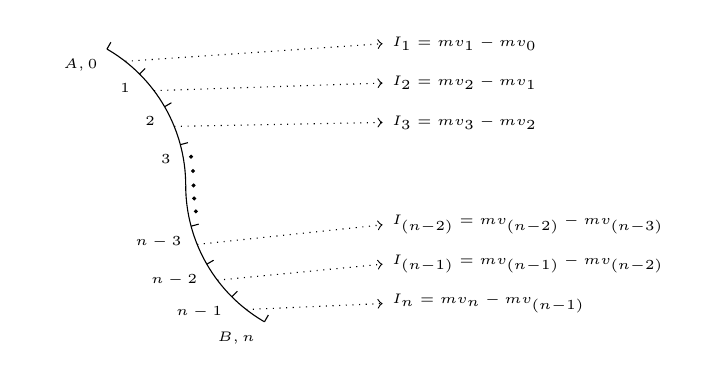
\begin{tikzpicture}
   \draw (0,0) arc (0:60:2); 
   \draw (0,0) arc (180:240:2);
   \draw (-2,0)+(60:2) node [anchor= north east]{\tiny $A,0$}--+(60:2.1);
   \draw (-2,0)+(45:2) node [anchor= north east]{\tiny $1$}--+(45:2.1);
   \draw (-2,0)+(30:2) node [anchor= north east]{\tiny $2$}--+(30:2.1);
   \draw (-2,0)+(15:2) node [anchor= north east]{\tiny $3$}--+(15:2.1);
   \draw[->,dotted] (-2,0)+(52:2)--+(4.5,1.8) node [anchor=west]{\tiny $I_1=mv_1-mv_0$};
   \draw[->,dotted] (-2,0)+(37:2)--+(4.5,1.3) node [anchor=west]{\tiny $I_2=mv_2-mv_1$};
   \draw[->,dotted] (-2,0)+(22:2)--+(4.5,0.8) node [anchor=west]{\tiny $I_3=mv_3-mv_2$};
   \filldraw (-2,0)+(10:2.1) circle [radius=0.5pt]; 
   \filldraw (-2,0)+(5:2.1) circle [radius=0.5pt]; 
   \filldraw (-2,0)+(0:2.1) circle [radius=0.5pt]; 
   \filldraw (2,0)+(185:1.9) circle [radius=0.5pt]; 
   \filldraw (2,0)+(190:1.9) circle [radius=0.5pt]; 
   \draw (2,0)+(195:2) node [anchor= north east]{\tiny $n-3$}--+(195:1.9);
   \draw (2,0)+(210:2) node [anchor= north east]{\tiny $n-2$}--+(210:1.9);
   \draw (2,0)+(225:2) node [anchor= north east]{\tiny $n-1$}--+(225:1.9);
   \draw (2,0)+(240:2) node [anchor= north east]{\tiny $B,n$}--+(240:1.9);
   \draw[->,dotted]  (2,0)+(202:2)--+(0.5,-0.5) node [anchor=west] {\tiny $I_{(n-2)}=mv_{(n-2)}-mv_{(n-3)}$};
   \draw[->,dotted]  (2,0)+(217:2)--+(0.5,-1) node [anchor=west]   {\tiny $I_{(n-1)}=mv_{(n-1)}-mv_{(n-2)}$};
   \draw[->,dotted] (2,0)+(232:2)--+(0.5,-1.5) node [anchor=west]  {\tiny $I_n=mv_n-mv_{(n-1)}$};
 \end{tikzpicture}
  \caption{动量定理}
  \label{fig:dongliang}
\end{figure}

记总冲量为

\[
  I=I_1+I_2+I_3+\cdots +I_{(n-1)}+I_{(n)}
\]

注意:上式是各个部分冲量的矢量和,不是简单的代数相加.

则动量部分,错位相消,最后得到动量定理为

\begin{equation}
  I=mv_n-mv_0
  \label{eq:dldl2}
\end{equation}

令 $n\to \infty$ 则误差消失,通常我们用 $p'=mv_\infty$ 表示末动量,用 $p=mv$ 表示初动量,所以得到动量定理式 \eqref{eq:dldl} 即

\begin{equation}
  I=p'-p
\end{equation}


动量定理是一个矢量式,所以也可以在某一个方向上列出动量定理,例如

\begin{equation}
  I_x=P'_x-P_x
  \label{eq:dldlsub}
\end{equation}

\section{动量守恒定律}

动量守恒定律: 如果一个系统不受外力或所受合外力为零,则系统的动量守恒.

动量守恒定律的表达式为

\begin{equation}
  p'_1+p'_2+p'_3+\cdot p'_n = p_1+p_2+p_3+\cdots +p_n
  \label{eq:dlsh}
\end{equation}

上式中 $p'_i (i=1,2,3\cdots)$ 表示系统内各物体的末动量,$p_i (i=1,2,3\cdots)$ 表示系统内各物体的初动量.

下面以两个物体为例来介绍动量守恒定律.如果系统只包含两个物体 $m_1$ 和 $m_2$ ,如图\ref{fig:dlsh1}所示,图中 $F_{21}$ 表示 $m_2$ 对 $m_1$ 的力, $F_{12}$ 表示 $m_1$ 对 $m_2$ 的力,$F_1$ 表示 $m_1$ 受到的外力,$F_2$ 表示 $m_2$ 受到的外力.

\begin{figure}[H]
  \centering
  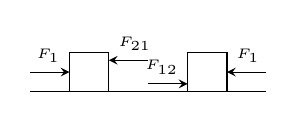
\begin{tikzpicture}
    \draw (-1,0) rectangle (-0.5,0.5);
    \draw (1,0) rectangle (0.5,0.5);
    \draw (-1.5,0)--(1.5,0);
    \draw [->,>=stealth] (0,0.4)--(-0.5,0.4) node [anchor=south west] {\tiny $F_{21}$};
    \draw [->,>=stealth] (0,0.1)--(0.5,0.1) node [anchor=south east] {\tiny $F_{12}$};
    \draw [->,>=stealth] (-1.5,0.25)--(-1,0.25) node [anchor=south east] {\tiny $F_1$};
    \draw [->,>=stealth] (1.5,0.25)--(1,0.25) node [anchor=south west] {\tiny $F_1$};
  \end{tikzpicture}
  \caption{动量守恒定律}
  \label{fig:dlsh1}
\end{figure}

分别对 $m_1$ 和 $m_2$ 写出动量定理

\begin{gather}
  (F_1+F_{21})t=p_1'-p_1 \label{eq:dlsh2a}\\
  (F_2+F_{12})t=p_2'-p_2 \label{eq:dlsh2b}
\end{gather}

将式 \eqref{eq:dlsh2a} 和式 \eqref{eq:dlsh2b} 相加,得

\begin{gather}
  (F_1+F_2+F_{12}+F_{21})t=(p_1'+p_2')-(p_1+p_2)
  \label{eq:xtdlsh}
\end{gather}

由 Newton 第三定律可得 $F_{12}+F_{21}=0$ ,所以上式化为

\begin{equation}
  (F_1+F_2)t=(p_1'+p_2')-(p_1+p_2)
  \label{eq:xtdlsh1}
\end{equation}

式 \eqref{eq:xtdlsh} 又称为 系统的动量定理.也就是,一个系统动量的变化等于所有外力的冲量的矢量和.

如果系统所受合外力为零或者不受外力,则$F_1+F_2=0$ 于是式 \eqref{eq:xtdlsh1} 为零,则移项后得

\begin{equation}
  p_1'+p_2'=p_1+p_2
  \label{eq:xtdlsh2}
\end{equation}

对于多个物体构成的系统,则用同样的方法可以得到式 \eqref{eq:dlsh},即系统的动量守恒定律.

在实际问题中,也常用到一种特殊的情况,就是内力远大于外力,此时动量近似守恒.对于解决碰撞和爆炸问题,相当方便.当 $F_{21}\gg F_1$ 和 $F_{12}\gg F_2$ 时,$m_1$ 和 $m_2$ 的动量定理可以用相当高的近似程度近似表达为

\begin{gather}
  F_{21}t=p_1'-p_1 \label{eq:dlsh2c}\\
  F_{12}t=p_2'-p_2 \label{eq:dlsh2d}
\end{gather}

同理,将\eqref{eq:dlsh2c} 和 \eqref{eq:dlsh2d} 相加,然后代入 Newton 第三定律可得动量守恒定律

\begin{equation*}
  p_1'+p_2'=p_1+p_2
\end{equation*}
